% coding:utf-8
\documentclass[a5paper,10pt,fleqn]{book}

\usepackage{fosa_layout}

\setboolean{ti}{true}        % Anleitung für TI-89
\setboolean{nspire}{true}    % Anleitung für TI-Nspire CAS
\setboolean{tiboth}{true}    % Anleitung für beide TR (Nur für Titelseite relevant)

\title{Formelsammlung Mathematik\\\textcolor{red}{\textbf{\Huge{Achtung! Dies ist noch nicht die definitive Version!}}}\\ Ab Samstag, 12.01.2013 15:00 liegt die fertige Version bereit. }
\ifti
\title{Formelsammlung Mathematik \\ Mit Anleitung zu TI-89\\\textcolor{red}{\textbf{\Huge Achtung! Dies ist noch nicht die definitive Version!}}\\ Ab Samstag, 12.01.2013 15:00 liegt die fertige Version bereit. }
\fi
\ifnspire
\title{Formelsammlung Mathematik \\ Mit Anleitung zu TI-Nspire\\\textcolor{red}{\textbf{\Huge{Achtung! Dies ist noch nicht die definitive Version!}}}\\ Ab Samstag, 12.01.2013 15:00 liegt die fertige Version bereit. }
\fi
\iftiboth
\title{Formelsammlung Mathematik \\ Mit Anleitung zu TI-89 und TI-Nspire CAS \\\textcolor{red}{\textbf{\Huge{Achtung! Dies ist noch nicht die definitive Version!}}}\\ Ab Samstag, 12.01.2013 15:00 liegt die fertige Version bereit. }
\fi

\author{Daniel Winz, Ervin Mazlagic, Adrian Imboden}
\date{\today~\dtc}


\begin{document}

\maketitle

% coding:utf-8
\chapter*{Über diese Arbeit}
Dies ist das Ergebnis einer Zusammenarbeit auf Basis freier Texte erstellt von Studierenden der Fachhochschule Luzern. 
\ifti
Zudem sind in dieser Formelsammlung Tipps und Hinweise für die Bedienung des TI-89 enthalten. 
\fi
\ifnspire
Zudem sind in dieser Formelsammlung Tipps und Hinweise für die Bedienung des TI-Nspire CAS enthalten. 
\fi
Dieses Schriftstück ist lizenziert unter der GPLv2 und der \TeX-  bzw. \LaTeX- Code ist auf \url{github.com/daniw/fosamath} hinterlegt.
Eine aktuelle PDF-Ausgabe ist auf \url{fosa.adinox.ch} abgelegt. 

%Leider können wir für nicht bestandene Prüfungen keine Haftung übernehmen. 

\tableofcontents

\chapter{Rechenregeln}
% coding:utf-8

%----------------------------------------
%FOSAMATH, a LaTeX-Code for a mathematical summary for basic analysis
%Copyright (C) 2013, Daniel Winz, Ervin Mazlagic, Adrian Imboden, Philipp Langer

%This program is free software; you can redistribute it and/or
%modify it under the terms of the GNU General Public License
%as published by the Free Software Foundation; either version 2
%of the License, or (at your option) any later version.

%This program is distributed in the hope that it will be useful,
%but WITHOUT ANY WARRANTY; without even the implied warranty of
%MERCHANTABILITY or FITNESS FOR A PARTICULAR PURPOSE.  See the
%GNU General Public License for more details.
%----------------------------------------

% coding:utf-8
\section{Rechenregeln}
\subsection{Bruchrechnen}
\[ \boxed{\frac{a}{b} \cdot \frac{c}{d} = \frac{a \cdot c}{b \cdot d}} \]
\[ \boxed{n \frac{a}{b} = \frac{n \cdot a}{b}} \]
\[ \boxed{\frac{a}{b} : \frac{c}{d} = \frac{a}{b} \cdot \frac{d}{c} = \frac{a \cdot d}{b \cdot c}} \]

\subsection{Polynomdivision}
Das Vorgehen bei der Polynomdivision ist identisch zur schriftlichen Division. \\\\
Beispiel: 
% \[ \boxed{\begin{array}{rrrlrl}
% &(9x^3 &- 6&x^2 &- 8x&):(3x + 4) = \underline{\underline{3x^2 + 2x}}\\
% -&(9x^3 &- 12&x^2)&&\\
% &&6&x^2 &- 8x&\\
% &&-(6&x^2 &- 8x&)\\
% &&&&0&
% \end{array}} \]

\begin{tabular}{|r@{}r@{}r@{}r@{}l@{}r@{}r@{}l|}
\hline
\rule{0pt}{12pt}&&$(9x^3 $&$- 6$&$x^2 $&$- 8x$&$)$&$:(3x + 4) = \underline{\underline{3x^2 + 2x}}$\\
&$-$&$(9x^3 $&$- 12$&$x^2)$&$\downarrow\,\,$&&\\
\cline{2-5}\rule{0pt}{12pt}&&&$6$&$x^2 $&$- 8x$&&\\
&&&$-(6$&$x^2 $&$- 8x$&$)$&\\
\cline{4-7}\rule{0pt}{12pt}&&&&&$0$&&\\
\hline
\end{tabular}


\subsection{Potenzen}
\[ \boxed{a^n = a \cdot a^{n-1} \quad a^1 = a} \]
\[ \boxed{a^0 = 1 \quad \left(0^0\right)\text{ ist nicht definiert}} \]
\[ \boxed{a^{-1} = \frac{1}{a}} \]
\[ \boxed{a^{-n} = \frac{1}{a^n}} \]

\subsection{Potenzgesetze}
\[ \boxed{a^x \cdot a^y = a^{x+y}} \]
\[ \boxed{\frac{a^x}{a^y} = a^{x-y}} \]
\[ \boxed{(a^x)^y = a^{xy}} \]
\[ \boxed{a^x \cdot b^x = \left(ab\right)^x} \]
\[ \boxed{\frac{a^x}{b^x} = \left(\frac{a}{b}\right)^x} \]
\[ \boxed{a^{\frac{p}{q}} = \sqrt[q]{a^p}} \]

\subsection{Wurzeln}
\[ \boxed{\sqrt[n]{a^m} = a^{\frac{m}{n}} \quad \left(a>0; m, n \in \mathbb{N}; m \geq 1; n \geq 2\right)} \]
\[ \boxed{\sqrt[n]{1}=1 \quad \sqrt[n]{0}=0 \quad \sqrt[n]{a^n}=a \quad \left(a>0\right)} \]

\subsection{Wurzelgesetze}
\[ \boxed{\sqrt[n]{a}\cdot \sqrt[n]{b}=\sqrt[n]{a\cdot b}} \]
\[ \boxed{\frac{\sqrt[n]{a}}{\sqrt[n]{b}}=\sqrt[n]{\frac{a}{b}}} \]
\[ \boxed{\left(\sqrt[n]{a}\right)^k=\sqrt[n]{a^k}} \]
\[ \boxed{\sqrt[nk]{a^{mk}}=\sqrt[n]{a^m}} \]
\[ \boxed{\sqrt[n]{\sqrt[m]{a}}=\sqrt[m]{\sqrt[n]{a}}=\sqrt[mn]{a}} \]

\subsection{Logarithmengesetze}
\[ \boxed{y=\log_ax \Leftrightarrow a^y=x} \]
\[ \boxed{\log_a1=0 \quad \log_aa=1} \]
\[ \boxed{\lg a=\log_{10}a \quad \ln a = \log_ea} \]
\[ \boxed{a^{\log_ax}=x} \]
\[ \boxed{\log_a\left(a^x\right)=x} \]
% \subsubsection{Produkte}
\[ \boxed{\log_b\left(x \cdot y\right) = \log_b\left(x\right) + \log_b\left(y\right)} \]
% \subsubsection{Quotienten}
\[ \boxed{\log_b \left( \frac{x}{y} \right) = \log_b\left(x\right) - \log_b\left(y\right)} \]
% \subsubsection{Summen und Differenzen}
%\[ \boxed{\log_b\left(x \cdot y\right) = \log_b\left(x\right) + \log_b\left(y\right)} \]
\[ \boxed{\log_b\left(x + y\right) = \log_b\left(x\right) + \log_b\left(1 + \frac{y}{x}\right)} \]
% \subsubsection{Potenzen}
\[ \boxed{\log_b\left(x^r\right) = r \cdot \log_b\left(x\right)} \]
\[ \boxed{\log_ax=\frac{\lg x}{\lg a}=\frac{\ln x}{\ln a}} \]

\newpage
\subsection{Trigonometrie}

\begin{figure}[h!]
\centering
\includegraphics[width=0.9\textwidth]{einheitskreis.pdf}
\end{figure}

\newpage
\noindent
$H$: Hypotenuse\\
$A$: Ankathete\\
$G$: Gegenkathete
\[ \boxed{\sin\alpha=\frac{G}{H}} \quad \boxed{\cos\alpha=\frac{A}{H}} \quad \boxed{\tan\alpha=\frac{G}{A}} \quad \boxed{\cot\alpha=\frac{A}{G}} \]
\[ \boxed{\sin x = \sqrt{1-\cos^2x} = \sqrt{\frac{\tan^2x}{1+\tan^2x}}} \]
\[ \boxed{\cos x = \sqrt{1-\sin^2x} = \sqrt{\frac{1}{1+\tan^2x}}} \]
\[ \boxed{\tan x = \frac{\sin x}{\sqrt{1-\sin^2x}} = \frac{\sqrt{1-\cos^2x}}{\cos x} = \frac{\sin x}{\cos x}} \]
\[ \boxed{\sin^2 x + \cos^2 x = 1} \]

\subsection{Spezielle Werte der Winkelfunktionen}
% \begin{tabular}{|l|c|c|c|c|c|}
% \hline              & 0°$ = 0$ & 30°$ = \frac{\pi}{6}$ & 45°$ = \frac{\pi}{4}$ & 60°$ = \frac{\pi}{3}$ & 90°$ = \frac{\pi}{2}$ \\
% \hline $f\left(x\right)=\sin x$ & $0$ & $\frac{1}{2}$ & $\frac{1}{2}\sqrt{2}$ & $\frac{1}{2}\sqrt{3}$ & $1$ \\
% \hline $f\left(x\right)=\cos x$ & $1$ & $\frac{1}{2}\sqrt{3}$ & $\frac{1}{2}\sqrt{2}$ & $\frac{1}{2}$ & $0$ \\
% \hline $f\left(x\right)=\tan x$ & $0$ & $\frac{1}{3}\sqrt{3}$ & $1$ & $\sqrt{3}$ & nicht def. \\
% \hline $f\left(x\right)=\cot x$ & nicht def. & $\sqrt{3}$ & $1$ & $\frac{1}{3}\sqrt{3}$ & $0$ \\
% \hline \end{tabular}

% \begin{tabular}{|l||r|r|r|r|}
% \hline $\varphi$                    &          $\sin(\varphi)$&          $\cos(\varphi)$&          $\tan(\varphi)$&          $\cot(\varphi)$\\
% \hline $0^\circ=0$                  &                      $0$&                      $1$&                      $0$&          nicht definiert\\
% \hline $30^\circ=\frac{\pi}{6}$     &            $\frac{1}{2}$&    $\frac{1}{2}\sqrt{3}$&    $\frac{1}{3}\sqrt{3}$&               $\sqrt{3}$\\
% \hline $45^\circ=\frac{\pi}{4}$     &    $\frac{1}{2}\sqrt{2}$&    $\frac{1}{2}\sqrt{2}$&                      $1$&                      $1$\\
% \hline $60^\circ=\frac{\pi}{3}$     &    $\frac{1}{2}\sqrt{3}$&            $\frac{1}{2}$&               $\sqrt{3}$&    $\frac{1}{3}\sqrt{3}$\\
% \hline $90^\circ=\frac{\pi}{2}$     &                      $1$&                      $0$&          nicht definiert&                      $0$\\
% \hline $120^\circ=\frac{2\pi}{3}$   &    $\frac{1}{2}\sqrt{3}$&           $-\frac{1}{2}$&              $-\sqrt{3}$&   $-\frac{1}{3}\sqrt{3}$\\
% \hline $135^\circ=\frac{3\pi}{4}$   &    $\frac{1}{2}\sqrt{2}$&   $-\frac{1}{2}\sqrt{2}$&                     $-1$&                     $-1$\\
% \hline $150^\circ=\frac{5\pi}{6}$   &            $\frac{1}{2}$&   $-\frac{1}{2}\sqrt{3}$&   $-\frac{1}{3}\sqrt{3}$&              $-\sqrt{3}$\\
% \hline $180^\circ=\pi$              &                      $0$&                     $-1$&                      $0$&          nicht definiert\\
% \hline $210^\circ=\frac{7\pi}{6}$   &           $-\frac{1}{2}$&   $-\frac{1}{2}\sqrt{3}$&    $\frac{1}{3}\sqrt{3}$&               $\sqrt{3}$\\
% \hline $225^\circ=\frac{5\pi}{4}$   &   $-\frac{1}{2}\sqrt{2}$&   $-\frac{1}{2}\sqrt{2}$&                      $1$&                      $1$\\
% \hline $240^\circ=\frac{4\pi}{3}$   &   $-\frac{1}{2}\sqrt{3}$&           $-\frac{1}{2}$&               $\sqrt{3}$&    $\frac{1}{3}\sqrt{3}$\\
% \hline $270^\circ=\frac{3\pi}{2}$   &                     $-1$&                      $0$&          nicht definiert&                      $0$\\
% \hline $300^\circ=\frac{5\pi}{3}$  &   $-\frac{1}{2}\sqrt{3}$&            $\frac{1}{2}$&              $-\sqrt{3}$&   $-\frac{1}{3}\sqrt{3}$\\
% \hline $315^\circ=\frac{7\pi}{4}$   &   $-\frac{1}{2}\sqrt{2}$&    $\frac{1}{2}\sqrt{2}$&                     $-1$&                     $-1$\\
% \hline $330^\circ=\frac{11\pi}{6}$  &           $-\frac{1}{2}$&    $\frac{1}{2}\sqrt{3}$&   $-\frac{1}{3}\sqrt{3}$&              $-\sqrt{3}$\\
% \hline $360^\circ=2 \pi$            &                      $0$&                      $1$&                      $0$&          nicht definiert\\
% \hline\end{tabular}

\[ \begin{array}{|l||r|r|r|r|}
\hline \varphi                    &          \sin(\varphi)&          \cos(\varphi)&          \tan(\varphi)&          \cot(\varphi)\\
\hline 0^\circ=0                  &                      0&                      1&                      0& \text{nicht definiert}\\
\hline 30^\circ=\frac{\pi}{6}     &            \frac{1}{2}&    \frac{1}{2}\sqrt{3}&    \frac{1}{3}\sqrt{3}&               \sqrt{3}\\
\hline 45^\circ=\frac{\pi}{4}     &    \frac{1}{2}\sqrt{2}&    \frac{1}{2}\sqrt{2}&                      1&                      1\\
\hline 60^\circ=\frac{\pi}{3}     &    \frac{1}{2}\sqrt{3}&            \frac{1}{2}&               \sqrt{3}&    \frac{1}{3}\sqrt{3}\\
\hline 90^\circ=\frac{\pi}{2}     &                      1&                      0& \text{nicht definiert}&                      0\\
\hline 120^\circ=\frac{2\pi}{3}   &    \frac{1}{2}\sqrt{3}&           -\frac{1}{2}&              -\sqrt{3}&   -\frac{1}{3}\sqrt{3}\\
\hline 135^\circ=\frac{3\pi}{4}   &    \frac{1}{2}\sqrt{2}&   -\frac{1}{2}\sqrt{2}&                     -1&                     -1\\
\hline 150^\circ=\frac{5\pi}{6}   &            \frac{1}{2}&   -\frac{1}{2}\sqrt{3}&   -\frac{1}{3}\sqrt{3}&              -\sqrt{3}\\
\hline 180^\circ=\pi              &                      0&                     -1&                      0& \text{nicht definiert}\\
\hline 210^\circ=\frac{7\pi}{6}   &           -\frac{1}{2}&   -\frac{1}{2}\sqrt{3}&    \frac{1}{3}\sqrt{3}&               \sqrt{3}\\
\hline 225^\circ=\frac{5\pi}{4}   &   -\frac{1}{2}\sqrt{2}&   -\frac{1}{2}\sqrt{2}&                      1&                      1\\
\hline 240^\circ=\frac{4\pi}{3}   &   -\frac{1}{2}\sqrt{3}&           -\frac{1}{2}&               \sqrt{3}&    \frac{1}{3}\sqrt{3}\\
\hline 270^\circ=\frac{3\pi}{2}   &                     -1&                      0& \text{nicht definiert}&                      0\\
\hline 300^\circ=\frac{5\pi}{3}   &   -\frac{1}{2}\sqrt{3}&            \frac{1}{2}&              -\sqrt{3}&   -\frac{1}{3}\sqrt{3}\\
\hline 315^\circ=\frac{7\pi}{4}   &   -\frac{1}{2}\sqrt{2}&    \frac{1}{2}\sqrt{2}&                     -1&                     -1\\
\hline 330^\circ=\frac{11\pi}{6}  &           -\frac{1}{2}&    \frac{1}{2}\sqrt{3}&   -\frac{1}{3}\sqrt{3}&              -\sqrt{3}\\
\hline 360^\circ=2 \pi            &                      0&                      1&                      0& \text{nicht definiert}\\
\hline\end{array} \]


\subsection{Quadratische Gleichung}
\[ \boxed{f(x) = a \cdot x^2 + b \cdot x + c} \]
\[ \boxed{x_{1,2}=\frac{-b\pm\sqrt{b^2-4ac}}{2a}} \]

\subsection{Binomische Formeln}
Erste Binomische Formel: 
\[ \boxed{(a + b)^2 = a^2 + 2 \cdot a \cdot b + b^2} \]Zweite Binomische Formel: 
\[ \boxed{(a - b)^2 = a^2 - 2 \cdot a \cdot b + b^2} \]Dritte Binomische Formel: 
\[ \boxed{(a + b) \cdot (a - b) = a^2 - b^2} \]

\subsection{Verkettete Funktionen}
\[ \boxed{(f \circ g)(x) := f(g(x))} \]

\subsection{Grenzwerte}
\[ \boxed{\lim\limits_{x \to x_0}(f_1(x) + f_2(x)) = \lim\limits_{x \to x_0}(f_1(x)) + \lim\limits_{x \to x_0}(f_2(x))} \]
\[ \boxed{\lim\limits_{x \to x_0}(f_1(x) - f_2(x)) = \lim\limits_{x \to x_0}(f_1(x)) - \lim\limits_{x \to x_0}(f_2(x))} \]
\[ \boxed{\lim\limits_{x \to x_0}(f_1(x) \cdot f_2(x)) = \lim\limits_{x \to x_0}(f_1(x)) \cdot \lim\limits_{x \to x_0}(f_2(x))} \]
\[ \boxed{\lim\limits_{x \to x_0}\left(\frac{f_1(x)}{f_2(x)}\right) = \frac{\lim\limits_{x \to x_0}(f_1(x))}{\lim\limits_{x \to x_0}(f_2(x))}} \]
\[ \boxed{\lim\limits_{x \to x_0}(c \cdot f_1(x)) = c \cdot \lim\limits_{x \to x_0}(f_1(x))} \]
\[ \boxed{\lim\limits_{x \to x_0}\left(c^{(f_1(x))}\right) = c^{\left(\lim\limits_{x \to x_0}(f_1(x))\right)}} \]
\[ \boxed{\lim\limits_{x \to x_0}\left((f_1(x))^n\right) = \left(\lim\limits_{x \to x_0}(f_1(x))\right)^n} \]
\[ \boxed{\lim\limits_{x \to x_0}\left(\sqrt[n]{(f_1(x))}\right) = \sqrt[n]{\lim\limits_{x \to x_0}(f_1(x))}} \]
\[ \boxed{\lim\limits_{x \to x_0}\left(\log{(f_1(x))}\right) = \log{\lim\limits_{x \to x_0}(f_1(x))}} \]

\subsection{Berechnung von Grenzwerten}
Um Grenzwerte zu ermitteln muss der Ausdruck so angepasst werden, dass eindeutig bestimmt werden kann, was sich daraus ergibt.
Dies wird durch Anwenden der zuvor aufgezeigten Rechenreglen erreicht.\\\\
Bsp.: $ \quad \quad \lim\limits_{n \rightarrow \infty} \left( \dfrac{\alpha \cdot n^2}{n^2-1} \right) $ \\\\
Um den Grenzwert zu ermitteln muss der Ausdruck erweitert werden und zwar so, dass
\begin{itemize}
\item der Term äquivalent bleibt
\item Variabeln des Indizes entfallen
\end{itemize}
Um die geforderten Bedingungen zu erfüllen wird der Term durch den reziproken Wert des Indizes mit der höchsten Potenz (im Zähler!) erweitert. In diesem Fall mit $\frac{1}{n^2}$. 
Eine weitere Regel besagt, dass konstante Faktoren vorangenommen werden können.
Nun sieht es wie folgt aus:\\\\
\indent \indent \indent $ \alpha \lim\limits_{n \rightarrow \infty} 
    \left( \dfrac{\frac{1}{n^2} \cdot (n^2) }{ \frac{1}{n^2} \cdot (n^2 -1) } \right)  $\\\\\\
Vereinfacht man diesen Ausdruck durch elementare Algebra so erhält man: \\\\
\indent \indent \indent $ \alpha \lim\limits_{n \rightarrow \infty} \left( \dfrac{1}{1-
\smash{\underbrace{\frac{1}{n^2}}_0 } \vphantom{\dfrac{1}{n^2}} } \right) $\\\\\\
Der Audruck $\frac{1}{n^2}$ geht für $n \rightarrow \infty$ zu $0$. Daraus ergibt sich das folgende:\\\\\\
\indent \indent \indent $ \alpha \cdot 1 = \alpha $

\ifti
\subsubsection{Berechnung von Grenzwerten mit dem TI-89}\label{subsubsec:limti}
%limit($a_n$, $n$, $\infty)$
\verb?limit(EXP,VAR,POINT[,DIRECTION])?\\\\
\begin{tabular}{@{}lll}
\verb|EXP|	& Ausdruck	& bezeichnet den Term \\
\verb|VAR|	& Variable	& bezeichnet die Variable \\
\verb|POINT|	& Punkt		& bezeichnet den Variablenwert \\
\verb|DIRECTION|& Richtung 	& bezeichnet die Richtung \\
		&		& $\searrow$~~~~von oben: 1 \\
		&		& $\nearrow$~~~~von unten: -1 \\
\end{tabular}\\\\
Bsp.: \verb| limit((x^2-2)/(x-2),x,2,-1)| \\
\indent\indent erzeugt die Ausgabe $\mathtt{ \lim\limits_{x \rightarrow 2^-} (\dfrac{x^2-2}{x-2}) \quad = \quad - \infty } $
\fi
\ifnspire
\subsubsection{Berechnung von Grenzwerten mit dem TI-Nspire}\label{subsubsec:limnspire}
\[ \lim\limits_{\boxed{n}\to\boxed{\infty}^{\boxed{d}}}(\boxed{a_n}) \]\\
\begin{tabular}{@{}llp{6cm}}
$\boxed{a_n}$    & Ausdruck & bezeichnet den Term \\
$\boxed{n}$      & Variable & bezeichnet die Variable \\
$\boxed{\infty}$ & Punkt    & bezeichnet den Variablenwert \\
$\boxed{d}$      & Richtung & bezeichnet die Richtung \\
                 &          & $\searrow$ : von oben: + \\
                 &          & $\nearrow$ : von unten: - \\
		 &          & Wenn keine Richtung gefordert ist, kann dieses Feld leer gelassen werden. 
\end{tabular}
\fi

\subsubsection{L'Hopital}
Die Regel von L'Hopital besagt, dass wenn man einen Grenzwert der Form 
\[ \lim\limits_{x \rightarrow x_0} \frac{f(x)}{g(x)} \Rightarrow \lim\limits_{x \rightarrow x_0} f(x) = \lim\limits_{x \rightarrow x_0} g(x) = 0 \Rightarrow \lim\limits_{x \rightarrow x_0} \frac{0}{0} \] hat, kann der Grenzwert auch über die Ableitungen ermittelt werden, falls der Grenzwert existiert.
Erhält man wieder einen unbestimmten Ausdruck, so kann erneut die Regel von L'Hopital angewendet werden (dies kann man so oft wie nötig wiederholen).
\[ \boxed{ \lim\limits_{x \rightarrow x_0} \frac{f(x)}{g(x)} = \lim\limits_{x \rightarrow x_0} \frac{f'(x)}{g'(x)} \quad} \quad \text{falls Bedingungen erfüllt sind!}\]

\subsection{Fakultät}
\[ \boxed{K! = 1 \cdot 2 \cdot 3\cdot \ldots \cdot K} \qquad \boxed{0! := 1} \]
\[ \boxed{(K + 1)! = 1  \cdot 2 \cdot \ldots \cdot K \cdot (K + 1) = (K + 1) \cdot K!} \]
\[ \boxed{(K - 1)! = 1  \cdot 2 \cdot \ldots \cdot (K - 1) = 1  \cdot 2 \cdot \ldots \cdot (K - 1) \cdot \frac{K}{K} = \frac{K!}{K}} \]
\subsubsection{Einige Fakultäten}
\[ \boxed{\begin{array}{rcr}
\rowcolor{white}  0!&=&1\\
\rowcolor{lgray}  1!&=&1\\
\rowcolor{white}  2!&=&2\\
\rowcolor{lgray}  3!&=&6\\
\rowcolor{white}  4!&=&24\\
\rowcolor{lgray}  5!&=&120\\
\rowcolor{white}  6!&=&720\\
\rowcolor{lgray}  7!&=&5'040\\
\rowcolor{white}  8!&=&40'320\\
\rowcolor{lgray}  9!&=&362'880\\
\rowcolor{white} 10!&=&3'628'800\\
\rowcolor{lgray} 11!&=&39'916'800\\
\rowcolor{white} 12!&=&479'001'600\\
\rowcolor{lgray} 13!&=&6'227'020'800\\
\rowcolor{white} 14!&=&87'178'291'200\\
\rowcolor{lgray} 15!&=&1'307'674'368'000\\
\rowcolor{white} 16!&=&20'922'789'888'000\\
\rowcolor{lgray} 17!&=&355'687'428'096'000\\
\rowcolor{white} 18!&=&6'402'373'705'728'000\\
\rowcolor{lgray} 19!&=&121'645'100'408'832'000\\
\rowcolor{white} 20!&=&2'432'902'008'176'640'000\\
\end{array}}\]

% coding:utf-8

%----------------------------------------
%FOSAMATH, a LaTeX-Code for a mathematical summary for basic analysis
%Copyright (C) 2013, Daniel Winz, Ervin Mazlagic, Adrian Imboden, Philipp Langer

%This program is free software; you can redistribute it and/or
%modify it under the terms of the GNU General Public License
%as published by the Free Software Foundation; either version 2
%of the License, or (at your option) any later version.

%This program is distributed in the hope that it will be useful,
%but WITHOUT ANY WARRANTY; without even the implied warranty of
%MERCHANTABILITY or FITNESS FOR A PARTICULAR PURPOSE.  See the
%GNU General Public License for more details.
%----------------------------------------

% coding:utf-8
\section{Darstellung von Funktionen}
\subsection{Polares Koordinatensystem}
Eine Funktion kann auch im Polaren Koordinatensystem definiert werden. 
Dabei wird jeder Punkt durch den Abstand zur Ordinate und den Winkel zur x-Achse definiert. 

\begin{figure}[h!]
\includegraphics[width=1\textwidth]{polar.pdf}
\end{figure}

% \begin{figure}[h!]
%\includegraphics[height=1\textwidth,angle=270]{polar_2.pdf}
%\end{figure}

\subsection{Umrechnung Kartesisch $\rightarrow$ Polar}
\[ \boxed{r = \sqrt{x^2 + y^2}} \]
\[ \boxed{\varphi = \arctan\left(\frac{y}{x}\right)} \]

\subsection{Umrechnung Polar $\rightarrow$ Kartesisch}
\[ \boxed{x = r \cdot \cos{\varphi}} \]
\[ \boxed{y = r \cdot \sin{\varphi}} \]

\subsection{Parameterdarstellung}
Bei der Paramaterdarstellung wird jeder Punkt durch die x- und die y-Koordinate definiert. 
\[ \boxed{f(t) = \left(\begin{matrix} x(t)\\ y(t) \end{matrix}\right)} \] 

\noindent 
Weitere Informationen zur Ableitung in der Parameterdarstellung siehe~\ref{subsec:ableitungsregeln} (Seite \pageref{subsec:ableitungsregeln})


\chapter{Vektorgeometrie}
% coding:utf-8
\section{Vektorgeometrie in der Ebene}

\subsection{Abstand zweier Puntke}
\[ \boxed{ \overline{P_1 P_2} = \sqrt{ (x_2 - x_1)^2 + (y_2 - y_1)^2 } } \]

\subsection{Geradengleichungen}

\subsubsection{Normalform (explizite Form)}
\[ \boxed{ g: y= mx + q }\]
\[ \boxed{ \text{Steigung } m = \frac{y_2 - y_1}{x_2 - x_1} = \frac{\Delta y}{\Delta x}  = tan \varphi } \]

\subsubsection{Koordinatenform (implizite Form)}
\[ \boxed{ g: ax + by + c = 0 } \]

\subsubsection{Achsenabschnittsform}
\[ \boxed{ g: \frac{x}{p} + \frac{y}{q} = 1 } \]

\subsubsection{Hesse'sche Normalform}
\[ \boxed{ g:  \frac{ax + by + c}{\sqrt{ a^2 + b^2 } } = 0 }  \]

\subsubsection{Parameterform}
\[ \boxed{ 
	g: \vec{r} = \vec{r_0} + t \cdot \vec{a}  = 
    \left( 
		\begin{array}{cc} 
	  		x_0 \\ y_0
		\end{array}
	\right)
    + t \cdot 
    \left( 
		\begin{array}{cc} 
			a_x \\ a_y
		\end{array}
    \right)  
   }
\]


\subsection{Normalenvektor}
Der Normalenvektor ist ein Vektor, welcher senkrecht auf einem anderen Vektor bzw. einer Geraden liegt. Hier im Beispiel in welchem $ \vec{n} \bot g(x)$
\[ \boxed{ \vec{n} = 
	\left( 
		\begin{array}{cc} 
	  		n_x \\ n_y
		\end{array}
    \right)
    =
    \left( 
		\begin{array}{cc} 
			a \\ b
		\end{array}
    \right)
    =
    \left( 
		\begin{array}{cc} 
			-a_y \\ a_x
		\end{array}
    \right)
} \]
\noindent
Der Richtungsvektor von $g(x)$ ist 
$  
	\left( 
		\begin{array}{cc} 
	  		a_x \\ a_y
		\end{array}
    \right)
    \Rightarrow 
    \left( 
		\begin{array}{cc} 
	  		-a_y \\ a_x
		\end{array}
    \right)
    = \vec{n}
$.

\subsection{Abstand Punkt zu Gerade}
Für eine Gerade $g: ax + by + c = 0$ und einen Punkt $P_1 (x_1 | y_1)$ gilt:
\[ \boxed{ d = \left| \frac{ax_1 + by_1 + c}{\sqrt{a^2 + b^2}} \right| } \]

\subsection{Schnittwinkel zwischen Geraden}
Für den spitzen Schnittwinkel $\varphi$ zwischen den Geraden 

$g_1: y = m_1x + q_1$ und $g_2: y = m_2x + q_2$ gilt:
\[ \boxed{ tan\varphi = \left| \frac{m_2 - m_1}{1 + m_1 \cdot m_2} \right| } \\ \text{für } \varphi \neq 90^{\circ} \]

\[ \boxed{ g_1 || g_2 \Leftrightarrow m_1 = m_2 \text{und } g_1 \bot g_2 \Leftrightarrow m_2 = - \frac{1}{m_1} } \\ \text{für } m_1 \neq 0 \]

\section{Vektorgeometrie im Raum}

\subsection{Ortsvektor}
Ein Ortsvektor beschreibt den Vektor vom Urspung des Koordinatensystems $O(0|0|0)$ zu einem beliebigen Punkt $P(x|y|z)$.
\[	\boxed{ \vec{r} = \overrightarrow{OP} = x\vec{e_x} + y\vec{e_y} + z\vec{e_z} :=
	\left( 
	  \begin{array}{ccc} 
	    x \\ y \\ z
	  \end{array}
	\right) }
\]
\noindent
Die Vektoren $\vec{e_x},\vec{e_y},\vec{e_z}$ sind die Einheitsvektoren des Koordinatensystems (meist einfach 1 ohne Einheit).
\subsection{Länge eines Ortsvektors (Norm bzw. Betrag)}
\[ \boxed{ ||\vec{r}|| = r = \sqrt{x^2 + y^2 + z^2} } \]

\subsection{Länge eines Vektors (Norm bzw. Betrag)}
\[ \boxed{ ||\vec{a}|| = a = \overrightarrow{P_1P_2} = \sqrt{a_x^2 + a_y^2 + a_z^2} } \]
In dieser Form entspricht $a$ der Raumdiagonale im Quader zu $(a_x|a_y|a_z)$.

\subsection{Vektor aus Anfangs- und Endpunkt}
Möchte man den Vektor $\vec{a}$ von $P_1$ (Anfangspunkt) zu $P_2$ (Endpunkt) haben, so rechnet man Anfang - Ende, bzw. $\vec{P_2} - \vec{P_1}$.
\[  \boxed{
    \vec{a} = \overrightarrow{P_1P_2} = \vec{r_2} - \vec{r_1} =
    \left( 
	  \begin{array}{ccc} 
	    x_2 - x_1 \\ y_2 - y_1 \\ z_2 - z_1
	  \end{array}
	\right)
    }
\]

\subsection{Distanz zweier Punkte}
Um die Distanz von $P_1$ zu $P_2$ zu ermitteln, berechnet man die Norm von $\overrightarrow{P_1P_2}$.
\[ \boxed{
   \overline{P_1P_2} = \sqrt{ (x_2 - x_1)^2 + (y_2 - y_1)^2 + (z_2 + z_1)^2 }
   }
\]

\subsection{Mittelpunkt einer Strecke}
\[ \boxed{ \vec{r_M} = \frac{1}{2} \cdot (\vec{r_1} + \vec{r_2}) } \]
\[ \boxed{ \Rightarrow x_M = \frac{x_1 + x_2}{2} \\ y_m = \frac{y_1 + y_2}{2} \\ z_M = \frac{z_1 + z_2}{2} } \]

\section{Rechenoperationen mit Vektoren}

\subsection{Addition/Subtraktion}
\[ \boxed{ \vec{a}\pm\vec{b} =  
    \left( 
	  \begin{array}{ccc} 
	    a_x \\ a_y \\ a_z
	  \end{array}
	\right)
	\pm
	\left( 
	  \begin{array}{ccc} 
	    b_x \\ b_y \\ b_z
	  \end{array}
	\right)
	=
	\left( 
	  \begin{array}{ccc} 
	    a_x \pm b_x \\ a_y \pm b_y \\ a_z \pm b_z
	  \end{array}
	\right)
} \]

\subsection{Multiplikation mit Skalar}
\[ \boxed{ k \cdot \vec{a} = k \cdot 
\left( 
	  \begin{array}{ccc} 
	    a_x \\ a_y \\ a_z
	  \end{array}
	\right)
	=
	\left( 
	  \begin{array}{ccc} 
	    k \cdot a_x \\ k \cdot a_y \\ k \cdot a_z
	  \end{array}
	\right)
	} \\ \text{für } k \in \mathbb{R}
\]

\subsection{Skalarprodukt}
\[ \boxed{ \vec{a} \cdot \vec{b} = a \cdot b \cdot cos(\varphi) = a_x b_x + a_y b_y + a_z b_z } \]
Der Winkel $\varphi$ ist der Zwischenwinkel von $\vec{a}$ und $\vec{b}$.

\noindent
Für $\vec{a} \neq \vec{0}$, $\vec{b} \neq \vec{0}$ gilt: $\vec{a} \bot \vec{b} \Leftrightarrow \vec{a} \cdot \vec{b} = 0$!

\subsection{Winkel zwischen zwei Vektoren}
\[ \boxed{ cos \varphi = \frac{\vec{a} \cdot \vec{b} }{||\vec{a}|| \cdot ||\vec{b}||} } \]
\[ \boxed{ cos \varphi = \frac{a_x b_x + a_y b_y + a_z b_z}{ \sqrt{a_x^2 + a_y^2 + a_z^2} \sqrt{b_x^2 + b_y^2 + b_z^2} } } \]

\subsection{Vektorprodukt (Kreuzprodukt)}
Mit dem Vektorprodukt erhält man einen Vektor der senkrecht zur Ebene steht, also den Normalenvektor zur Ebene.

\[ \boxed{ \vec{c} = \vec{a} \times \vec{b} = 
\left( 
	  \begin{array}{ccc} 
	    a_x \\ a_y \\ a_z
	  \end{array}
	\right)
	\times
	\left( 
	  \begin{array}{ccc} 
	    b_x \\ b_y \\ b_z
	  \end{array}
	\right)
	=
	\left( 
	  \begin{array}{ccc} 
	    a_y b_z - a_z b_y \\ a_z b_x - a_x b_z \\ a_x b_y - a_y b_x
	  \end{array}
	\right)
} \]
\noindent
Die Fläche die von $\vec{a}$ und $\vec{b}$ aufgespannt wird, entspricht der Norm des Vektorprodukts $c=|\vec{a}\times\vec{b}| = a \cdot b \cdot sin \varphi$ .
Zu Beachten ist, dass $\vec{b} \times \vec{a} = -(\vec{a} \times \vec{b}) $

\subsection{Spatprodukt}
Das Spatprodukt entspricht dem Volumen welches von drei Vektoren aufgespannt wird.

\[ \boxed{ (\vec{a},\vec{b},\vec{c}) = (\vec{a} \times \vec{b}) \cdot \vec{c} = (\vec{b} \times \vec{c}) \cdot \vec{a} = (\vec{c} \times \vec{a}) \cdot \vec{b} } \]


\chapter{Folgen und Reihen}
% coding:utf-8
\section{Folgen}
$a_1$ ist das erste Glied einer Folge\\
$a_n$ ist das $n$-te Glied einer Folge

\subsection{rekursive Darstellung}
Bei der rekursiven Darstellung wird eine Folge durch einen Startwert und eine Abbildungsvorschrift dargestellt. \\
\[ \boxed{ \begin{matrix}
\text{Startwert} & f(1) = a_1 \\
\text{Vorschrift} & F(f(1), f(2), \ldots, f(n)) := f(n + 1) = a_{n + 1}
\end{matrix}} \]

\subsection{arithmetische Folgen}
$d$ ist die Differenz zwischen zwei benachbarten Gliedern\\
\[ \boxed{a_{n+1} - a_n = d} \]
\[ \boxed{a_{n+1} = a_n + d} \]
\[ \boxed{ \begin{matrix} 
a_0 :& a_n =& a_0 + n \cdot d \\
a_1 :& a_n =& a_1 + (n - 1)d 
\end{matrix}}\]

\subsection{geometrische Folgen}
$q$ ist der Quotient von zwei benachbarten Gliedern\\
\[ \boxed{\frac{a_{n+1}}{a_n} = q} \]
\[ \boxed{a_{n+1} = a_n * q} \]
\[ \boxed{a_n = q^{n-1} a_1} \]

\subsection{Konvergenz von Folgen}

% coding:utf-8

%----------------------------------------
%FOSAMATH, a LaTeX-Code for a mathematical summary for basic analysis
%Copyright (C) 2013, Daniel Winz, Ervin Mazlagic, Adrian Imboden, Philipp Langer

%This program is free software; you can redistribute it and/or
%modify it under the terms of the GNU General Public License
%as published by the Free Software Foundation; either version 2
%of the License, or (at your option) any later version.

%This program is distributed in the hope that it will be useful,
%but WITHOUT ANY WARRANTY; without even the implied warranty of
%MERCHANTABILITY or FITNESS FOR A PARTICULAR PURPOSE.  See the
%GNU General Public License for more details.
%----------------------------------------

% coding:utf-8
\section{Reihen}
$S_n$ ist die Summe aller Glieder von $a_1$ bis $a_n$. 
\[ \boxed{S_n = \sum_{k=1}^{n} a_k = a_1 + a_2 + a_3 \cdots + a_n} \]

\subsection{arithmetische Reihe}
\[ \boxed{S_n = \left(n + 1\right)\left(a_0 + d \frac{n}{2}\right) = \left(n + 1\right) \frac{a_0 + a_n}{2}} \]

\subsection{geometrische Reihe}
\[ \boxed{\text{Für } q \neq 1: \quad S_n = a_1 \left(  \frac{q^n - 1}{q - 1} \right) = a_1 \left(  \frac{1 - q^n}{1 - q} \right)} \]

\[ \boxed{\begin{array}{ll}
a_0 :& S_n = a_0 \cdot \dfrac{1-q^{n+1}}{1-q} \\ 
& \\
a_1 :& S_n = a_1 \cdot \dfrac{1-q^n}{1-q}
\end{array}} \]

\[ \boxed{\text{Für } q = 1: \quad S_n = a_1 \left(1+1^1 + 1^2 + \ldots + 1^{n-1}\right) = a_1 n} \]
Unendliche geometrische Reihe
\[ \boxed{\text{Für } |q| < 1: S = \lim_{n \rightarrow \infty} S_n = \frac{a_1}{1 - q}} \] 
%Um das $n$-te Glied einer geometrischen Reihen zu berechnen gilt:\\
%$ q = \frac{a_n}{a_{n-1}} = \frac{a_{n-1}}{a_{n-2}} $ \\
%$ \Rightarrow  a_n = a_{(n-1)} \cdot q = a_{(n-2)} \cdot q^2 = a_{(n - (n-1))} \cdot q^{(n-1)} = a_1 \cdot q^{(n-1)} $
%\[ \boxed{ a_n = a_1 \cdot q^{n-1} } \]
%\[ \boxed{ a_{n+1} = a_1 \cdot q^n } \]
$a_1$ ist hier das erste Element der geometrischen Folge!

\subsection{Konvergenz}

\subsubsection*{Quotientenkriterium}
Um die Konvergenzfrage einer geometrischen Reihe zu klären betrachtet man
\[\boxed{ \lim\limits_{n \rightarrow \infty} \left| \frac{a_{n+1}}{a_n} \right| = \lim\limits_{n \rightarrow \infty} \left| q \right|} \]
Hierbei können drei verschiedene Ergebnisse entstehen:
\[ \boxed{\begin{array}{ll}
|q| < 1 & \text{die Reihe konvergiert} \\
|q| > 1 & \text{die Reihe divergiert} \\
|q| = 1 & \text{keine Aussage möglich}
\end{array}} \]
Dies wird oft als Quotientenkriterium bezeichnet.

\subsubsection*{Wurlzelkrierium}
Eine weitere Methode zur Klärung der Konvergenzfrage liefert das so genannte Wurzelkriterium.
\[\boxed{ \lim\limits_{n \rightarrow \infty} \left( |a_k| \right)^{\frac{1}{n}} = q }\]
Daraus können wie beim Quotientenkriterium drei Fälle eintreten:
\[ \boxed{\begin{array}{ll}
|q| < 1 & \text{die Reihe konvergiert} \\
|q| > 1 & \text{die Reihe divergiert} \\
|q| = 1 & \text{keine Aussage möglich} 
\end{array}} \]


\ifti
\subsection{Reihen mit dem TI89 berechnen}
$\sum$\verb{(Ausdruck,Variable,untere Grenze, obere Grenze){ \\
$\sum$\verb{(EXP,VAR,LOW,HIGH){ \\\\
\begin{tabular}{lll}
EXP  & Ausdruck      & bezeichnet den Term der die Reihe beschreibt \\
VAR  & Variable      & bezeichnet die inkrementierte Variable \\
LOW  & untere Grenze & Anfangspunkt der Inkrementierung \\
HIGH & obere Grenze  & Endpunkt der Inkrementierung \\
\end{tabular}
\fi
\ifnspire
\subsection{Reihen mit dem TI-Nspire berechnen}
\[ \sum_{\boxed{K} ~=~ \boxed{0}}^{\boxed{n}}\boxed{a_n} \]\\
\begin{tabular}{lll}
$\boxed{a_n}$  & Ausdruck      & bezeichnet den Term der die Reihe beschreibt \\
$\boxed{K}$     & Variable      & bezeichnet die inkrementierte Variable \\
$\boxed{0}$    & untere Grenze & Anfangspunkt der Inkrementierung \\
$\boxed{n}$ & obere Grenze  & Endpunkt der Inkrementierung \\
\end{tabular}
\fi


\chapter{Differenzieren}
% coding:utf-8
\section{Ableitungsregeln}

\subsection{Grundoperationen}

\subsubsection{Summenregel}
\[ \boxed{ (f(x) + g(x))' = f'(x) + g'(x) } \]
\[ \text{Wichtig: Ableitung einer konstanten Funktion ist Null! } \]
\[ \Rightarrow (f(x) + c)' = f'(x) \text{ für } c \in R \]

\subsubsection{Faktorregel}
\[ \boxed{ (c \cdot f(x))' = c \cdot f'(x) } \]
\[ \text{Ein konstanter Faktor bleiobt beim Differenzieren (Ableiten) erhalten!} \]

\subsubsection{Produkteregel}
\[ \boxed{ (f(x) \cdot g(x))' = f'(x) \cdot g(x) + f(x) \cdot g'(x) } \]

\subsubsection{Quotientenregel}
\[ \boxed{ \left( \frac{f(x)}{g(x)} \right) = \frac{ f'(x) \cdot g(x) - f(x) \cdot g'(x) }{ g^2(x) } } \\ \text{ gilt falls }g(x) \neq 0 \text{ !} \]

\subsubsection{Kettenregel}
\[ \boxed{ (f(g(x)))' = g'(x) \cdot f'(g(x)) } \]

\newpage

\subsection{Spezielle Regeln}

\subsubsection{Exponenten}
\[ \boxed{ (x^n)' = n\cdot x^{(n-1)} } \]
\[ \boxed{ (e^x)' = e^x } \]
\[ \boxed{ (e^{k\cdot x})' = k \cdot e^x } \]
\[ \boxed{ (a^x)' = ln_a (a^x) } \]

\subsubsection{Logarithmen}
\[ \boxed{ (ln(x))' = \frac{1}{x} } \]  
% \[ \boxed{ (a_{log_x})' = \frac{1}{x \cdot ln(a)} } \]

\subsubsection{Trigonometrie}
\[ \boxed{ (sin(x))' = cos(x) } \]  
\[ \boxed{ (cos(x))' = -sin(x) } \] 
\[ \boxed{ (tan(x))' = \frac{1}{cos^2(x)} } \]  
\[ \boxed{ (cot(x))' = -\frac{1}{sn^2(x)} } \]
% coding:utf-8
\section{Kurvendiskussion}

\subsection{Tangentengleichnung}
\[ \boxed{T(x) = f'(x_0)(x - x_0) + f(x_0)} \]

\subsection{Normale zur Tangente}
\[ \boxed{ T(x) = \frac{-1}{f'(x_0)} \cdot (x-x_0) + f(x_0) } \]

\subsection{Steigen und Fallen}

\[ \boxed{ \begin{array}{lll}
f'(x) \geq 0 \text{ auf } I & \Rightarrow  & f \text{ ist monoton wachsend in $I$} \\
f'(x) \leq 0 \text{ auf } I & \Rightarrow  & f \text{ ist monoton fallend in $I$} \\
f'(x) > 0 \text{ auf } I & \Rightarrow  & f \text{ ist streng monoton wachsend in $I$} \\
f'(x) < 0 \text{ auf } I & \Rightarrow  & f \text{ ist streng monoton fallend in $I$}
\end{array} } \]

\noindent
$I$ entspricht einem Intervall! Dies bedeutet, ist $f'(x)$ über den gesamten Bereich immer $\geq 0$ so ist $f$ monoton wachsend.
Ist $f'(x)$ über den gesamten Bereich $\leq 0$ so ist sie monoton fallend.

\subsection{Krümmungsverhalten}

\[ \boxed{ \begin{matrix}
f''(x) > 0 \text{ auf } I & \Rightarrow  & \text{ Kurve ist konvex } \\
f''(x) < 0 \text{ auf } I & \Rightarrow  & \text{ Kurve ist konkav }
\end{matrix} } \]

\subsection{Extremum}
Ein Extremum ist ein Punkt, zu welchem die Ableitung $0$ ergibt.
Solch ein Extremum kann ein Maximum oder Minimum sein.
Zusätzlich ist zu definieren ob es sich um ein lokales oder globales Extremum handelt.

\[ \boxed{ \begin{matrix}
f'(x_0) = 0 \land f''(x_0) < 0 & \Rightarrow & \text{lokales Maximum in $x_0$} \\
f'(x_0) = 0 \land f''(x_0) > 0 & \Rightarrow & \text{lokales Minimum in $x_0$} 
\end{matrix} } \]

\subsection{Wendepunkt}
Als Wendepukt bezeichnet man jene Stelle, an welcher die Krümmung der Funktion wechselt (konkav zu konvex und umgekehrt).
Im Wendepunkt ist die Steigung jeweils von beiden Seiten aus betrachtet (d.h aus $x_0 > 0$ und $x_0<0$) extremal.

\subsubsection{Notwendiges Kriterium}
\[ \boxed{ \begin{matrix}
f''(x_0) = 0 & \Rightarrow & \text{Wendepunkt in $x_0$}
\end{matrix} } \]

\subsubsection{Hinreichendes Kriterium}
\[ \boxed{ \begin{matrix}
f''(x_0) = 0 \land f'''(x_0) \neq 0 & \Rightarrow & \text{Wendepunkt in $x_0$}
\end{matrix} } \]
Achtung: Ist die dritte Ableitung 0, so kann an dieser Stelle trotzdem ein Wendepunkt sein. 

\subsection{Sattelpunkt}
Ein Sattelpunkt ist ein Wendepunkt mit horizontaler Wendetangente.

\[ \boxed{ \begin{matrix}
f'(x_0) =  f''(x_0) = 0 \land f'''(x_0) \neq 0 & \Rightarrow & \text{Sattelpunkt in $x_0$}
\end{matrix} } \]
% coding:utf-8



%----------------------------------------

%FOSAMATH, a LaTeX-Code for a mathematical summary for basic analysis

%Copyright (C) 2013, Daniel Winz, Ervin Mazlagic, Adrian Imboden, Philipp Langer



%This program is free software; you can redistribute it and/or

%modify it under the terms of the GNU General Public License

%as published by the Free Software Foundation; either version 2

%of the License, or (at your option) any later version.



%This program is distributed in the hope that it will be useful,

%but WITHOUT ANY WARRANTY; without even the implied warranty of

%MERCHANTABILITY or FITNESS FOR A PARTICULAR PURPOSE.  See the

%GNU General Public License for more details.

%----------------------------------------


% coding:utf-8

\section{Krümmung}

Die Krümmung $\kappa$ misst wie stark eine Kurve $\gamma$ gekrümmt ist (vgl. Kreis hat eine konstante Krümmung).
Die Krümmung wird unterschieden in mittlere und momentane Krümmung.
\[ \begin{array}{ll}
	\text{mittlere}  & \dfrac{\Delta \alpha}{\Delta s} \\
	& \\
	\text{momentane} & \dfrac{\delta \alpha}{\delta s} \\
\end{array} \]

\[ \boxed{r(t) = \dfrac{1}{|\kappa(t)|} \quad \quad \text{bzw.} \quad \quad r(x) = \dfrac{1}{|\kappa(x)|} } \]
\[ \boxed{\kappa(x) = \frac{y''(x)}{(1 + y'(x)^2)^{\frac{3}{2}}} }\]

\[\boxed{\begin{array}{lllll} 
	\kappa (x) > 0 & \rightarrow & y''(x) \stackrel{!}{>} 0 & \rightarrow & y \text{ ist konvex} \\
	\kappa (x) < 0 & \rightarrow & y''(x) \stackrel{!}{<} 0 & \rightarrow & y \text{ ist konkav} \\
	\kappa (x) = 0 & \rightarrow & y''(x) = 0		& \xrightarrow[]{Achtung!} & \text{Wendepunkt!}
\end{array}}\]
\section{Scheitelpunkte}
Scheitelpunkte sind Stellen an denen die Krümmung maximal ist. 
Um diese zu berechnen muss die Krümmung $\kappa (x)$ abgeleitet und Null gesetzt werden.
\[ \kappa '(x) \stackrel{!}{=} 0  \]
\[ \boxed{\kappa '(x) = \dfrac{ y'''(x)(1+y'(x)^2)^{\frac{3}{2}} - y''(x) \frac{3}{2}(1+y'(x)^2)^{\frac{1}{2}} y''(x) 2y'(x) }{ (1+y'(x)^2)^3 } \stackrel{!}{=} 0 } \]


\chapter{Integral}
% coding:utf-8
\section{Integral}
% coding:utf-8
\section{Integrationsregeln}
\subsection{Partielles Integrieren}
\[ \boxed{\int f'(x) \cdot g(x) dx = f(x) \cdot g(x) - \int f(x) \cdot g'(x) dx} \]
\subsection{Substitutionsregel}
\[ \boxed{\int_{g(a)}^{g(b)} f(x) dx = \int_{a}^{b} g'(x) \cdot f(g(x)) dx} \]


\section{Volumen}
\subsection{Rotationsvolumen}
\[ \boxed{V_x = \pi \int_{x_1}^{x_2} f(x)^2 dx} \quad \text{Rotation um die x-Achse}\]
\[ \boxed{V_y = \pi \int_{y_1}^{y_2} f^{-1}(y)^2 dy} \quad \text{Rotation um die y-Achse}\]

\section{Mittelwertsatz der Integralrechnung}
\[ \boxed{\int_{a}^{b} f(x) dx = f(\xi)(b-a)} \]

\section{Bogenlänge}
\[ \boxed{S = \int_{a}^{b} \sqrt{1 + y'(x)^2} dx} \]

\section{Bogenlänge für Kurven}
\[ \boxed{S = \int_{t_1}^{t_2}\sqrt{\dot{x}^2 + \dot{y}^2} dt \quad ,\gamma(t) = \left(\begin{matrix}x(t)\\y(t)\end{matrix}\right), t_1, t_2 \in I} \]

\section{Bogenlängen mit Polarkoordinaten}
\[ \boxed{S = \int_{\varphi_1}^{\varphi_2}\sqrt{\dot{r}^2(\varphi) + r^2(\varphi)}d\varphi} \]

\section{Mantelfläche}
\[ \boxed{A_{M_x} = 2 \pi \int_{x_1}^{x_2}f(x) \sqrt{1 + f'(x)^2} dx} \quad \text{Rotation um die x-Achse} \]
\[ \boxed{A_{M_y} = 2 \pi \int_{y_1}^{y_2}f^{-1}(y) \sqrt{1 + \frac{d}{dy}f^{-1}(y)^2} dy} \quad \text{Rotation um die y-Achse} \]

\section{Mantelfläche einer Kurve}
\[ \boxed{A_{M_x} = 2 \pi \int_{t_1}^{t_2} y(t) \sqrt{\dot{x}^2 + \dot{y}^2}dt} \quad \text{Bei Rotation um die x-Achse} \]
\[ \boxed{A_{M_y} = 2 \pi \int_{t_1}^{t_2} x(t) \sqrt{\dot{x}^2 + \dot{y}^2}dt} \quad \text{Bei Rotation um die y-Achse} \]

\section{Mantelfläche im polaren Koordinatensystem}
\[ \boxed{A_{M_x} = 2 \pi \int_{\varphi_1}^{\varphi_2}r(\varphi) \sin(\varphi)\sqrt{\dot{r}^2(\varphi) + r^2(\varphi)}} \quad \text{Bei Rotation um die x-Achse} \]
\[ \boxed{A_{M_y} = 2 \pi \int_{\varphi_1}^{\varphi_2}r(\varphi) \cos(\varphi)\sqrt{\dot{r}^2(\varphi) + r^2(\varphi)}} \quad \text{Bei Rotation um die y-Achse} \]

% coding:utf-8

%----------------------------------------
%FOSAMATH, a LaTeX-Code for a mathematical summary for basic analysis
%Copyright (C) 2013, Daniel Winz, Ervin Mazlagic, Adrian Imboden, Philipp Langer

%This program is free software; you can redistribute it and/or
%modify it under the terms of the GNU General Public License
%as published by the Free Software Foundation; either version 2
%of the License, or (at your option) any later version.

%This program is distributed in the hope that it will be useful,
%but WITHOUT ANY WARRANTY; without even the implied warranty of
%MERCHANTABILITY or FITNESS FOR A PARTICULAR PURPOSE.  See the
%GNU General Public License for more details.
%----------------------------------------


% coding:utf-8
\section{Ableitungen und unbestimmte Integrale spezieller Funktionen}
Integrationskonstante C ist weggelassen\\\\
\footnotesize
% \begin{tabular}{|c|c|c|}
% \hline \rule{80pt}{0pt} & \rule{80pt}{0pt} & \rule{80pt}{0pt} \\
% \textbf{$f'(x)$} & \textbf{$f(x)$} & \textbf{$\int f(x) dx$}\\&&\\
% \hline $0$ & $c \quad c \in \mathbb{R}$ & $cx$ \\
% \hline $c$ & $cx$ & $\frac{c}{2}x^2$ \\
% \hline $r \cdot x^{r-1}$ & $x^r \quad r \in \mathbb{R} \backslash \{-1\}$ & $\frac{x^{r+1}}{r+1}$ \\
% \hline $-\frac{1}{x^2} = -x^{-2}$ & $\frac{1}{x} = x^{-1}$ & $ln{|x|}$ \\
% \hline $\frac{1}{2\sqrt{x}} = \frac{1}{2}x^{-\frac{1}{2}}$ & $\sqrt{x} = x^{\frac{1}{2}}$ & $\frac{2}{3}x^{\frac{3}{2}}$ \\
% \hline $\cos x$ & $\sin x$ & $-\cos x$ \\
% \hline $-\sin x$ & $\cos x$ & $\sin x$ \\
% \hline $1 + \tan^2 x = \frac{1}{\cos^2 x}$ & $\tan x$ & $-\ln |\cos x|$ \\
% \hline $e^x$ & $e^x$ & $e^x$ \\
% \hline $c \cdot e^x$ & $e^{cx}$ & $\frac{1}{c} \cdot e^{cx}$ \\
% \hline $\ln a \cdot a^x$ & $a^x$ & $\frac{a^x}{\ln a}$ \\
% \hline $\frac{1}{x}$ & $\ln |x|$ & $x(ln |x| - 1)$ \\
% \hline $\frac{1}{ln a \cdot x}$ & $\log_a |x|$ & $\frac{x}{\ln a}(\ln |x| - 1) = x(\log_a |x| - \log_a e)$ \\
% \hline $\frac{1}{\sqrt{1 - x^2}}$ & $\arcsin x$ & $x \cdot \arcsin x + \sqrt{1 - x^2}$ \\
% \hline $-\frac{1}{\sqrt{1 - x^2}}$ & $\arccos x$ & $x \cdot \arccos x - \sqrt{1 - x^2}$ \\
% \hline $\frac{1}{1 + x^2}$ & $\arctan x$ & $x \cdot \arctan x - \frac{1}{2}\ln(1 + x^2)$ \\
% \hline \end{tabular}
% \\\\\\
\begin{equation*}
\begin{matrix}
f'(x) & f(x) & \int f(x) dx\\
\rule{0pt}{12pt}0 & c \quad c \in \mathbb{R} & cx \\
\rule{0pt}{12pt}c & cx & \frac{c}{2}x^2 \\
\rule{0pt}{12pt}r \cdot x^{r-1} & x^r \quad r \in \mathbb{R} \backslash \{-1\} & \frac{x^{r+1}}{r+1} \\
\rule{0pt}{12pt}-\frac{1}{x^2} = -x^{-2} & \frac{1}{x} = x^{-1} & ln{|x|} \\
\rule{0pt}{12pt}\frac{1}{2\sqrt{x}} = \frac{1}{2}x^{-\frac{1}{2}} & \sqrt{x} = x^{\frac{1}{2}} & \frac{2}{3}x^{\frac{3}{2}} \\
\rule{0pt}{12pt}\cos x & \sin x & -\cos x \\
\rule{0pt}{12pt}-\sin x & \cos x & \sin x \\
\rule{0pt}{12pt}1 + \tan^2 x = \frac{1}{\cos^2 x} & \tan x & -\ln |\cos x| \\
\rule{0pt}{12pt}e^x & e^x & e^x \\
\rule{0pt}{12pt}c \cdot e^x & e^{cx} & \frac{1}{c} \cdot e^{cx} \\
\rule{0pt}{12pt}\ln a \cdot a^x & a^x & \frac{a^x}{\ln a} \\
\rule{0pt}{12pt}\frac{1}{x} & \ln |x| & x(ln |x| - 1) \\
\rule{0pt}{12pt}\frac{1}{ln a \cdot x} & \log_a |x| & \frac{x}{\ln a}(\ln |x| - 1) = x(\log_a |x| - \log_a e) \\
\rule{0pt}{12pt}\frac{1}{\sqrt{1 - x^2}} & \arcsin x & x \cdot \arcsin x + \sqrt{1 - x^2} \\
\rule{0pt}{12pt}-\frac{1}{\sqrt{1 - x^2}} & \arccos x & x \cdot \arccos x - \sqrt{1 - x^2} \\
\rule{0pt}{12pt}\frac{1}{1 + x^2} & \arctan x & x \cdot \arctan x - \frac{1}{2}\ln(1 + x^2) \\
\end{matrix}
\end{equation*}
\normalsize


\chapter{Taylorreihen}
% coding:utf-8
\section{Taylorreihen}
Ein Ausdruck der Form 
\[ \boxed{f(x) = \sum_{K = 0}^{\infty} a_K x^K = a_0 + a_1 x + a_2 x^2 + a_3 x^3 \dots a_K x^K} \]
\[ \boxed{a_k = \frac{f^{(K)}(x_0)}{K!}} \]
nennt man eine Potenzreihe. \\\\
$f^{(K)}(x)$ ist dabei die K-te Ableitung von $f(x)$ gemeint. 

\subsection{Konvergenzradius}
Der Konvergenzradius sagt aus, innerhalb von welchem Intervall (ausgehend vom Approximationspunkt)
eine Potenzreihe konvergiert. Der Begriff Radius ist dabei ein Skalar auf $\Omega$ und nicht im $\mathbb{R}^2$.

\begin{figure}[h!]
\centering
\includegraphics[width=0.6\textwidth]{konvergenzradius.pdf}
\end{figure}

\[ \boxed{ \begin{array}{lll} 
    |x| < R & \Rightarrow & \text{Potenzreihe ist konvergent} \\
    |x| > R & \Rightarrow & \text{Potenzreihe ist divergent} \\
    |x| = R & \Rightarrow & \text{überprüfen was für $x=R$ und $-x=R$ gilt}
\end{array} } \]

\[ \boxed{R = \frac{1}{q} = \lim_{K \rightarrow \infty} \left| \frac{a_K}{a_{K + 1}} \right|} \]
% \quad \quad \text{wobei} \quad \quad a_k = \frac{f^{(K)}(x_0)}{K!} } \]

\subsection{Taylorreihe mit Entwicklungspunkt $x_0 = 0$}
Eine Taylorreihe mit Entwicklungspunkt $x_0 = 0$ wird auch MacLaurin-Reihe genannt
\[ \boxed{f(x) = \underbrace{\sum_{K=0}^{\infty}\frac{f^{(K)}(0)}{K!} x^K}_{\text{Taylorreihe}}} \]
\[ \boxed{f(x) = \underbrace{\sum_{K=0}^{n}\frac{f^{(K)}(0)}{K!} x^K}_{T_{(n,x_0)}(x)} + \underbrace{\sum_{K=n+1}^{\infty}\frac{f^{(K)}(0)}{K!} x^K}_{R_{n+1}(x)}} \]
$T_{(n,x_0)}(x)$ ist dabei das Taylorpolynom vom Grad n und $R_{n+1}(x)$ ist das Restglied. \\
Für das Restglied gilt: Es gibt eine Zahl $\xi$ zwischen $x_0$ und $x$ so, dass gilt: 
\[ \boxed{R_{n+1} = \frac{f^{(n + 1)}(\xi)}{(n + 1)!} \cdot (x - x_0)^{n + 1}} \]
Dies ist eine Restgliedformel (Lagrangsche Darstellung für $R_{n + 1}$). 

\subsection{Taylorreihe mit Entwicklungspunkt $x_0 \neq 0$}
\[ \boxed{f(x) = \sum_{K=0}^{\infty}\frac{f^{(K)}(x_0)}{K!}\cdot (x-x_0)^K} \]
\[ \boxed{f(x) = \underbrace{\sum_{K=0}^{n}\frac{f^{(K)}(x_0)}{K!} (x - x_0)^K}_{T_{(n,x_0)}(x)} + \underbrace{\sum_{K=n+1}^{\infty}\frac{f^{(K)}(x_0)}{K!} (x - x_0)^K}_{R_{n+1}(x)}} \]
$T_{(n,x_0)}(x)$ ist dabei das Taylorpolynom vom Grad n und $R_{n+1}(x)$ ist das Restglied. \\
Für das Restglied gilt: Es gibt eine Zahl $\xi$ zwischen $x_0$ und $x$ so, dass gilt: 
\[ \boxed{R_{n+1} = \frac{f^{(n + 1)}(\xi)}{(n + 1)!} \cdot (x - x_0)^{n + 1}} \]
Dies ist eine Restgliedformel (Lagrangsche Darstellung für $R_{n + 1}$). 

\subsection{Einfache Funktionen als Taylorreihen}
\[ \boxed{e^x = \sum_{K=0}^{\infty} \frac{x^K}{K!}} \]
\[ \boxed{\sin(x) = \sum_{K=0}^{\infty} \frac{(-1)^K x^{2K+1}}{(2K+1)!}} \]
\[ \boxed{\cos(x) = \sum_{K=0}^{\infty} \frac{(-1)^K x^{2K}}{(2K)!}} \]
\[ \boxed{\cosh(x) = \sum_{K=0}^{\infty} \frac{x^{2K}}{(2K)!}} \]
\[ \boxed{\sinh(x) = \sum_{K=0}^{\infty} \frac{x^{2K+1}}{(2K+1)!}} \]

\subsection{Kochrezept Taylorreihen}
\begin{enumerate}
  \item Stelle finden, an welcher die Funktion approximiert werden soll. 
  \item Bereich und Genauigkeit bzw. Fehler definieren oder den Grad der Potenzreihe fix wählen. 
  \item $a_0$, $a_1$, \dots $a_n$ berechnen. $n$ ist dabei der Grad der Potenzreihe
  \item Potenzreihe zusammensetzten
\end{enumerate}

\ifti
\subsection{Taylorreihe mit dem TI-89 berechnen}
\begin{verbatim}
taylor(Funktion,Variable,Ordnung[,Punkt])
\end{verbatim}
Funktion: Funktion, zu welcher die Taylorreihe gesucht ist. \\
Variable: Variable in Funktion\\
Ordnung: Ordnung der Taylorreihe\\
Punkt: Optional: Punkt, an dem Die Funktion approximiert wird. (Default: 0)
\fi
\ifnspire
\subsection{Taylorreihe mit dem TI-Nspire berechnen}
\begin{verbatim}
taylor(Funktion,Variable,Ordnung[,Punkt])
\end{verbatim}
Funktion: Funktion, zu welcher die Taylorreihe gesucht ist. \\
Variable: Variable in Funktion\\
Ordnung: Ordnung der Taylorreihe\\
Punkt: Optional: Punkt, an dem Die Funktion approximiert wird. (Default: 0)
\fi


\chapter{Fourierreihen}
% coding:utf-8

%----------------------------------------
%FOSAMATH, a LaTeX-Code for a mathematical summary for basic analysis
%Copyright (C) 2013, Daniel Winz, Ervin Mazlagic, Adrian Imboden, Philipp Langer

%This program is free software; you can redistribute it and/or
%modify it under the terms of the GNU General Public License
%as published by the Free Software Foundation; either version 2
%of the License, or (at your option) any later version.

%This program is distributed in the hope that it will be useful,
%but WITHOUT ANY WARRANTY; without even the implied warranty of
%MERCHANTABILITY or FITNESS FOR A PARTICULAR PURPOSE.  See the
%GNU General Public License for more details.
%----------------------------------------

% coding:utf-8
\section{Fourierreihen}

\subsection{gerade oder ungerade Funktionen}

\subsubsection{Gerade Funktion: }
\[ \boxed{f(-x) = f(x)} \]
Geometrisch gesehen, ist eine gerade Funktion an der y-Achse gespiegelt.
\subsubsection{Ungerade Funktion: }
\[ \boxed{f(-x) = -f(x)} \]
Geometrisch gesehen, ist eine ungerade Funktion am Ursprung gespiegelt.
\subsubsection{Achtung: }
Wichtig ist dabei, dass die Funktion erst nach der Erweiterung auf ganz $\mathbb{R}$ darauf geprüft wird, ob sie gerade oder ungerade ist. \\
So ist $\sin(x)$ eine ungerade Funktion. Wird jedoch nur die Periode $[0, \pi]$ betrachtet, so ist dies eine gerade Funktion.

\begin{figure}[h!]
\centering
\includegraphics[width=0.7\textwidth]{geradeungerade.pdf}
\end{figure}

\subsection{n-te Partialsumme für die Periode T}
\[ \boxed{f_n(x) = \frac{a_0}{2} + \sum_{K=1}^n \left(a_k \cdot \cos \left(\frac{2 \pi}{T} K x\right) + b_k \cdot \sin\left(\frac{2 \pi}{T} K x\right)\right)} \]

\subsection{Koeffizienten für die Periode T}
\[ \boxed{a_k = \frac{2}{T} \int_T f(x) \cos(\frac{2 \pi}{T} K x) dx} \]
\[ \boxed{b_k = \frac{2}{T} \int_T f(x) \sin(\frac{2 \pi}{T} K x) dx} \]
\[ \boxed{a_0 = \frac{2}{T} \int_T f(x) dx
} \]

\subsection{n-te Partialsumme einer Fourierreihe für die Periode 0 bis $2\pi$}
Die folgende Fourierreihe besitzt eine Periode von 0 bis 2 $\pi$.
Sie ist ein Spezialfall der oben beschriebenen Variante.
\[ \boxed{f_n(x) = \frac{a_0}{2} + \sum_{K=1}^n \left(a_k \cdot \cos(kx) + b_k \cdot \sin(Kx)\right)} \]

\subsection{Koeffizienten für die Periode $2\pi$}
\[ \boxed{a_k = \frac{1}{\pi} \int_0^{2 \pi} f(x) \cos(nx) dx} \]
\[ \boxed{b_k = \frac{1}{\pi} \int_0^{2 \pi} f(x) \sin(nx) dx} \]
\[ \boxed{a_0 = \frac{1}{\pi} \int_0^{2 \pi} f(x) dx
} \]
Ist $f$ eine ungerade Funktion d.h. $f(-x) = -f(x)$, so gilt, da der $\cos(x)$ eine gerade Funktion ist: 
\[ a_k \equiv 0 \quad \forall K\]
\[ a_0 \equiv 0 \]
Ist $f$ eine gerade Funktion: 
\[ b_k \equiv 0 \quad \forall K \]

\subsection{Kochrezept zu Fourierreihen}
\begin{enumerate}
  \item Periode bestimmen
  \item Funktion auf ganz $\mathbb{R}$ fortsetzen
  \item Bestimmung, ob gerade oder ungerade Funktion\\
  f ungerade: $a_0, a_k = 0$\\
  f gerade: $b_k = 0$
  \item $a_0, a_k$ und $b_k$ berechnen
  \item n-te trigonometrische Summe zu f hinschreiben
\end{enumerate}

\ifti
\subsection{Koeffizienzen der Fourierreihe mit dem TI-89 berechnen}
% \verb?integrate(?$\mathtt{\pi}$\verb?/2 * sin(@n1 * x),x,0,?$\mathtt{\pi}$\verb?)?\\
% $\mathtt{integrate\left(\frac{\pi}{2} \cdot sin(@n1 \cdot x), x, 0, \pi\right)}$\\
% $\text{integrate}\left(\frac{\pi}{2} \cdot \sin(@n1 \cdot x), x, 0, \pi\right)$
\verb?integrate(Ausdruck,Variable,untere Grenze, obere Grenze)? \\
\verb?integrate(EXPR,VAR[,LOW,UP])? \\\\
\begin{tabular}{@{}lll}
\verb?EXP?  & Ausdruck      & bezeichnet den Term der die Fourierreihe beschreibt \\
\verb?VAR?  & Variable      & bezeichnet die Variable, nach der integriert wird \\
\verb?LOW?  & untere Grenze & Anfangspunkt der Integration \\
\verb?HIGH? & obere Grenze  & Endpunkt der Integration \\
\end{tabular}\\
Für K wird \verb?@n1? eingegeben. 
\fi
\ifnspire
\subsection{Koeffizienten der Fourierreihe mit dem TI-Nspire berechnen}
\[ \int_{\boxed{0}}^{\boxed{\pi}}\boxed{\frac{\pi}{2}\sin(\mathtt{@n1} \cdot x)}~d\boxed{x} \]
$\mathtt{@n1}$ wird dabei anstelle von K eingegeben. Das $\mathtt{@}$ findet man dabei bei den Symbolen (Taste $\boxed{\boxed{^{\infty \beta ^\circ}}}$)
\fi


\end{document}

